\documentclass[a4paper]{paper}
\usepackage[utf8]{inputenc}
\usepackage[icelandic]{babel}
\usepackage[T1]{fontenc}
\usepackage{graphicx}
\usepackage{mathtools}
\usepackage{amsmath}
\usepackage{amssymb}
\usepackage{minted}
\usepackage{listings}
\usepackage{color}
\usepackage{wrapfig}

\definecolor{dkgreen}{rgb}{0,0.6,0}
\definecolor{gray}{rgb}{0.5,0.5,0.5}
\definecolor{mauve}{rgb}{0.58,0,0.82}

\lstset{frame=tb,
  language=Java,
  aboveskip=3mm,
  belowskip=3mm,
  showstringspaces=false,
  columns=flexible,
  basicstyle={\small\ttfamily},
  numbers=none,
  numberstyle=\tiny\color{gray},
  keywordstyle=\color{blue},
  commentstyle=\color{dkgreen},
  stringstyle=\color{mauve},
  breaklines=true,
  breakatwhitespace=true,
  tabsize=2
}

\graphicspath{ {./} }
\title{Snake}
\author{Þorvaldur Tumi Baldursson - ttb3@hi.is}

\begin{document}
\maketitle

\section{Inngangur}
Forritið er einföld útgáfa ef hinum klsassíska leik, Snake. 
Upphaflega var ég með mjög háfleygar hugmyndir um hverju ég gæti bætt við grunnleikinn en ég dembdi mér svo allharkalega í útlitslaugina og hafði því ekki tíma fyrir allt.
Það gerði það samt að verkum að leikurinn lítur mjög vel út, þrátt fyrir að ég segi sjálfur frá, og heldur þema allt í gegn.
Mesta vinnan við leikinn fór í að smíða kerfi til að halda utan um stöður "sprite-a" svo að snákurinn liðaðist rétt. 

\section{Þarfagreining}
\begin{center}
    \begin{tabular}{|l|l|p{6cm}|l|l|}
        \hline
        Nr.&Heiti&Lýsing&Týpa&Staða\\ \hline
        1.1&Liðun&Notandi getur spilað Snake þar sem snákurinn getur borðað mat,stækkað og liðast, 
        snákurinn deyr svo ef hann snertir eitursnák eða klessir á sinn eiginn líkama.&G&F\\ \hline
        1.2&Stigatafla&Notandi getur skráð stigin sín niður ásamt þremur einkennisstöfum,
        eins og í gömlum spilakössum. Þessi stig eiga að geymast á milli leikja.&G&F\\ \hline
        1.3&Ofurepli&Notandi getur hefnt sín á eitursnákum, öðru hvoru er maturinn sem birtist 'sérstakur'
        á þann hátt að þegar notandi borðar sérstaka matinn, 
        getur hann ekki dáið og ef snákurinn rekst á eitursnák deyr eitursnákurinn.
        Mjög svipuð pæling og stóru doppurnar í pac-man og stjörnur í super mario.&G&E\\ \hline
        1.4&Pása&Notandi getur pásað leik með mús, space eða escape. 
        Þegar notandi pásar leikinn fær viðkomandi yfirlit yfir hversu langur tími er liðinn,
        hversu mikinn mat er búið borða, hvar hann er í röðinni með stig á þessum tímapunkti, 
        hversu margir eitursnákar hafa birst, hversu margir eitursnákar hafa dáið og hversu mikið af sérstökum mat er búið að borða.&G&H\\ \hline
        1.5&Startskjár&Startskjár, 
        bæta við almennilegum startskjá þar sem hægt er að fá yfirlit yfir stig 
        og hugsanlega einhver auka skemmtileg gögn.&G&F\\ \hline
        2.1&Sprites&Allir leikjahlutir eiga að notast við sprites frekar en einföld form gerð í javafx.
        Það þarf ekki að vera sjúklegur munur á þessum spritum, 
        eitur og player snákar geta litið eins út nema með mismunandi litum.&Ú&F\\ \hline
        \end{tabular}
\end{center}

\section{Hönnun notendaviðmóts}
Ég hélt mig við hönnunina sem var gerð í verkefni 5, 
eina breytingin frá henni og lokaverkefninu er að þegar notandi deyr fer hann á skjá til að skrá stig frekar en það sem var sýnt í verkefni 5.
\begin{center}
    \begin{tabular}{c c}
        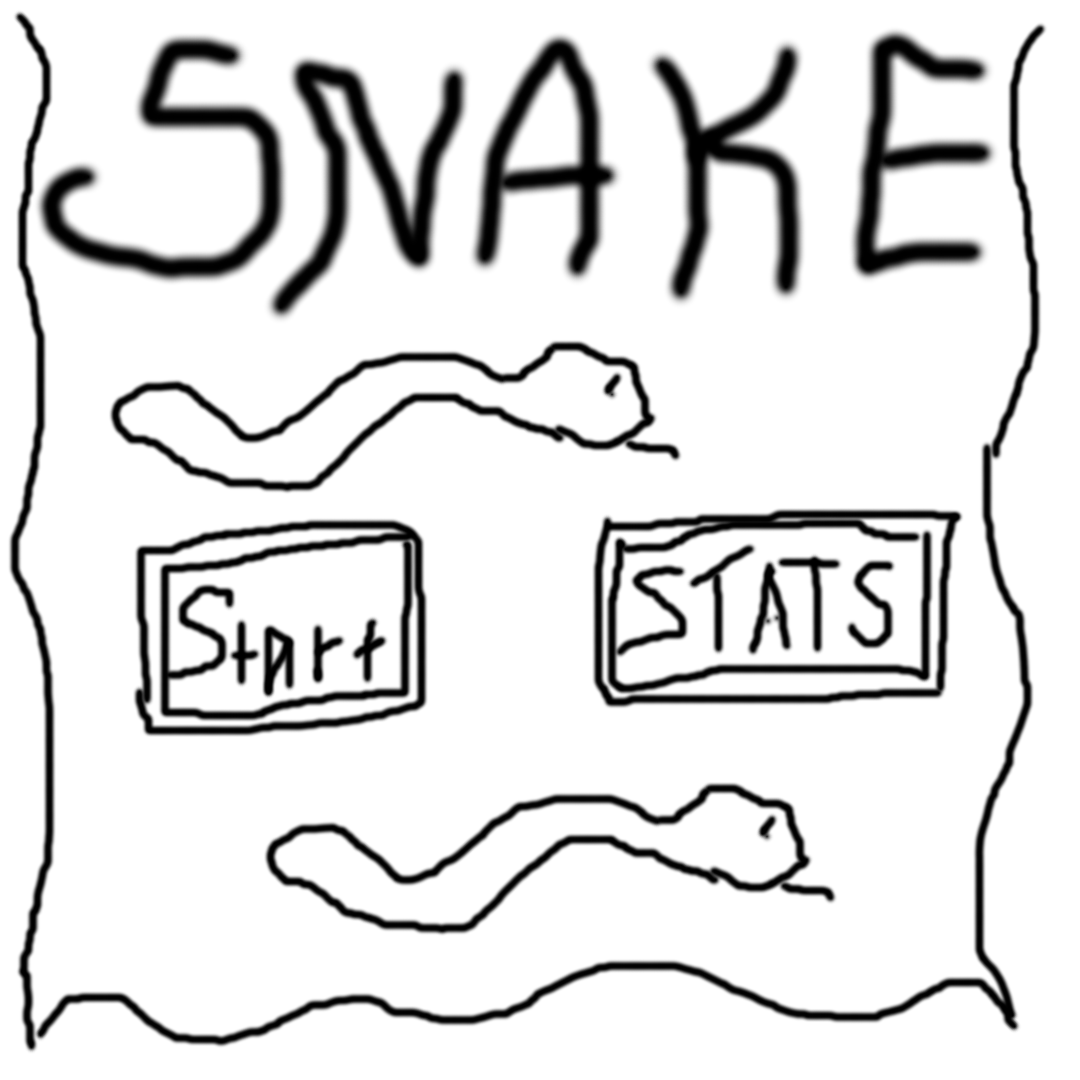
\includegraphics[scale=0.5]{imgs/m1.png}&
        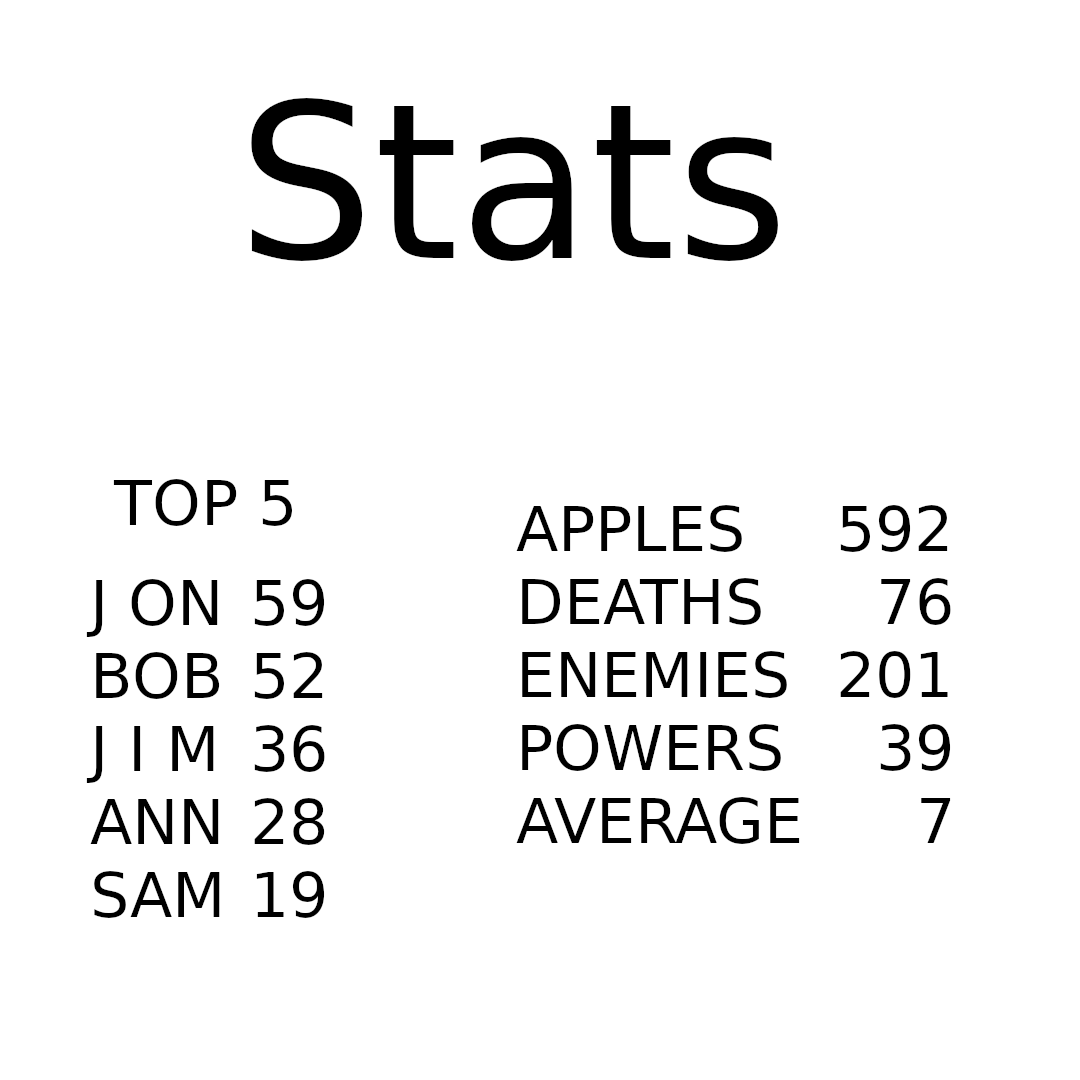
\includegraphics[scale=0.5]{imgs/m2.png}\\
        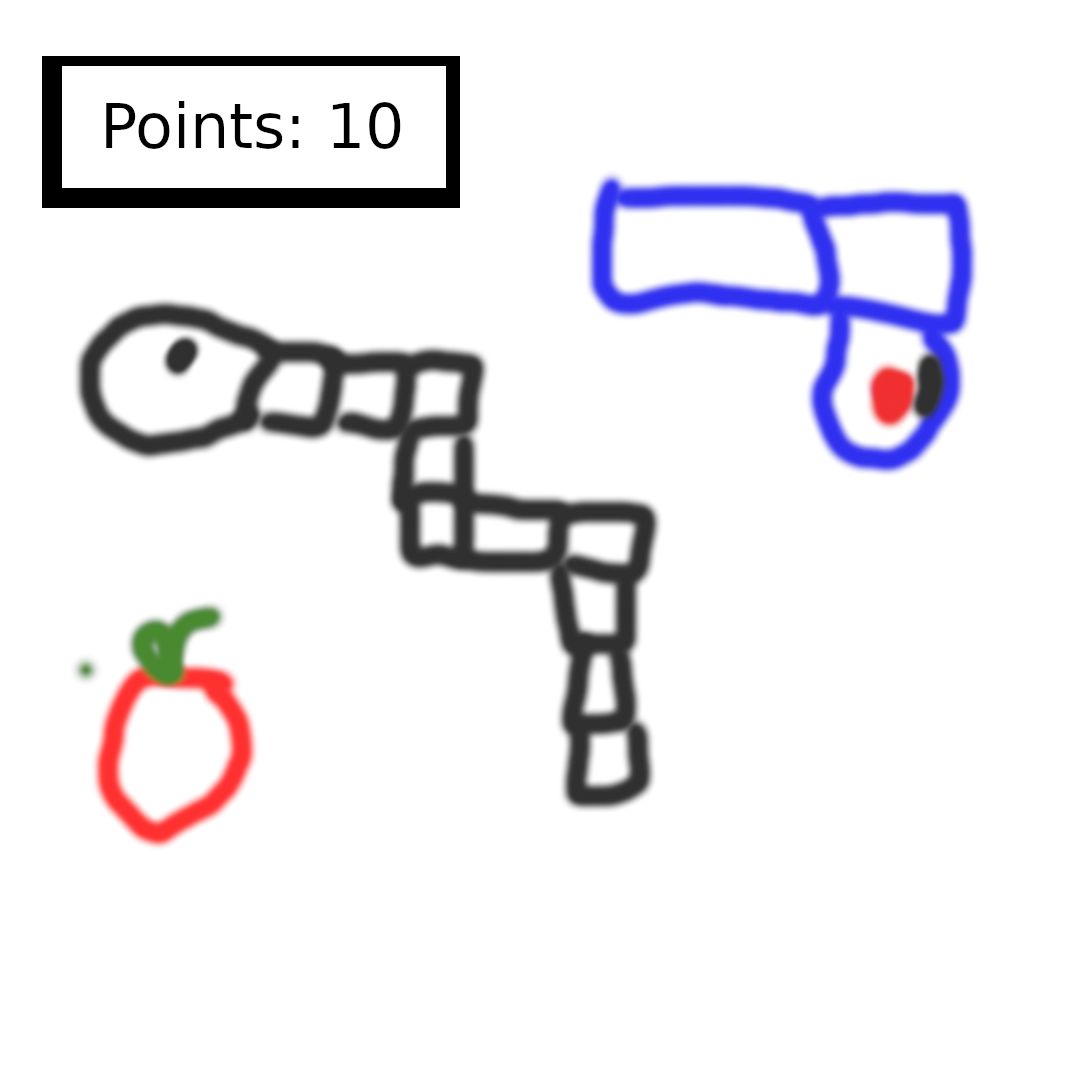
\includegraphics[scale=0.5]{imgs/m3.png}&
        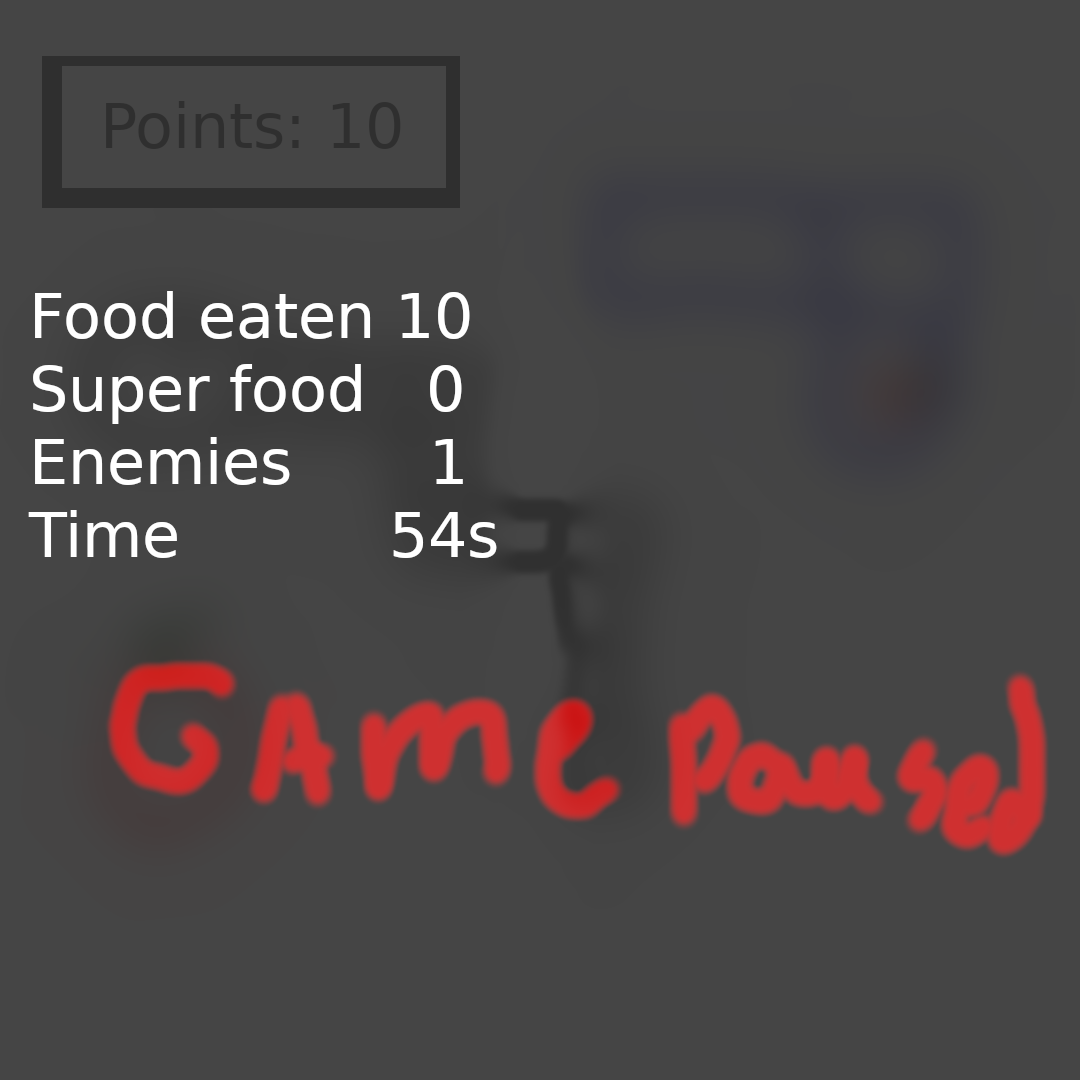
\includegraphics[scale=0.5]{imgs/m4.png}\\
        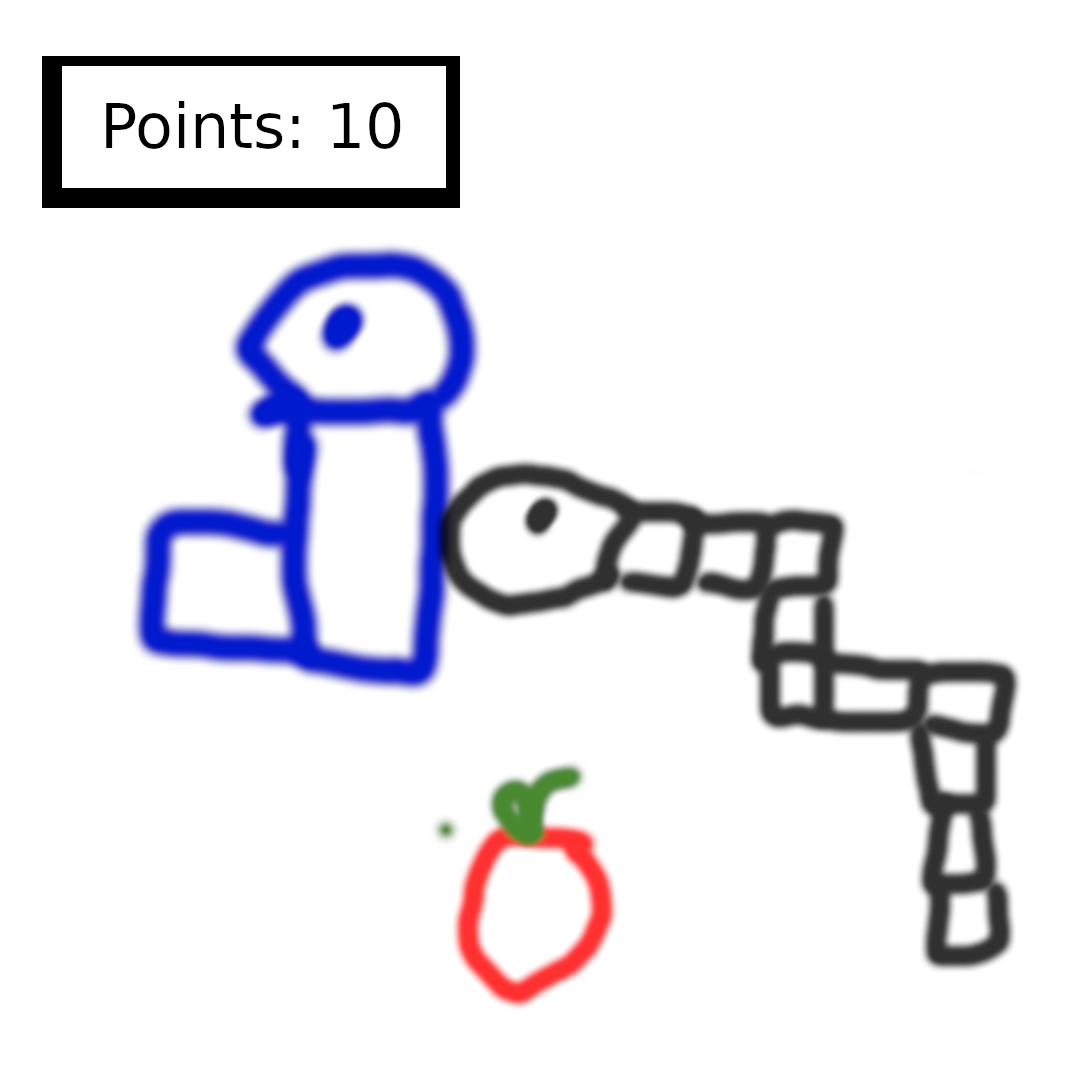
\includegraphics[scale=0.5]{imgs/m5.png}&
        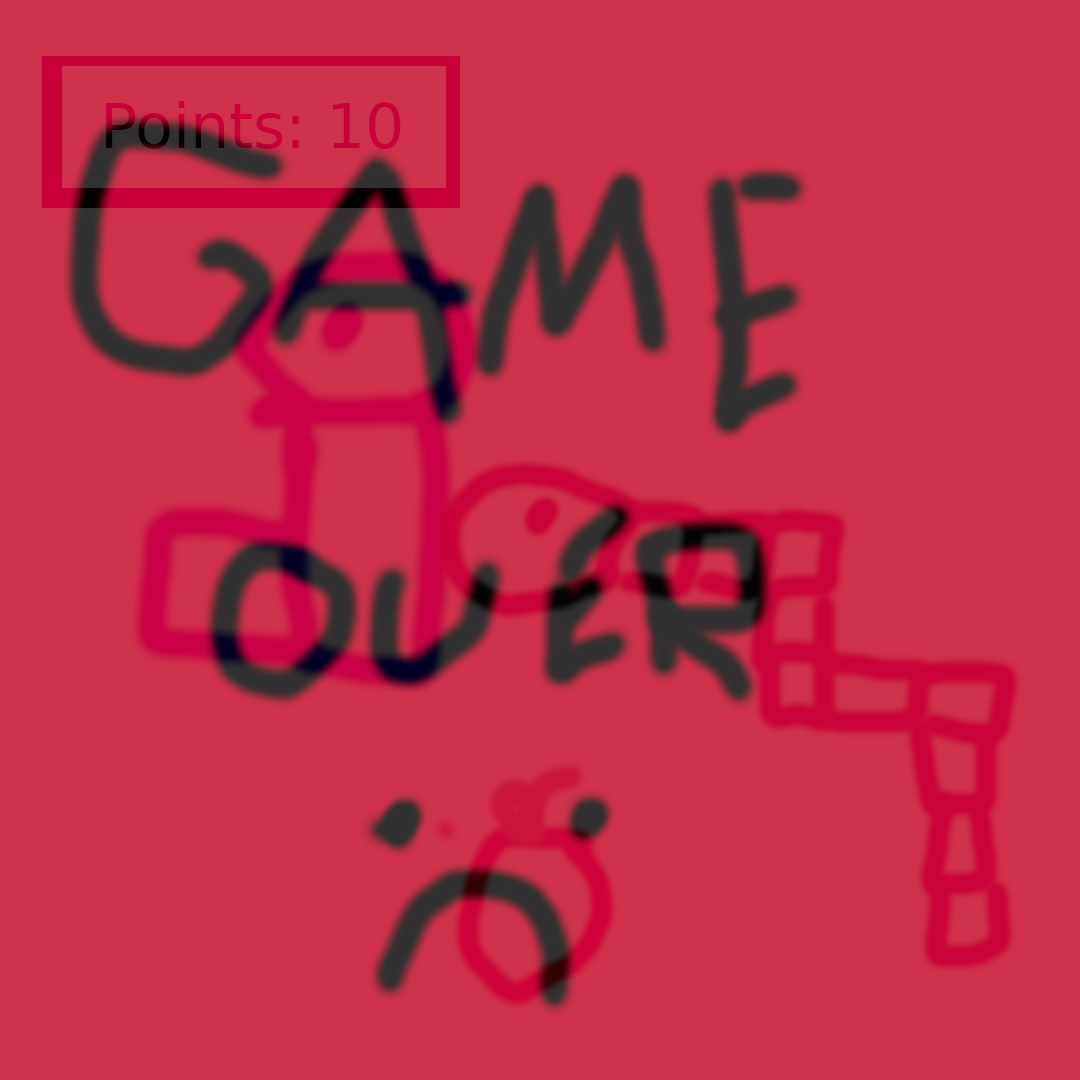
\includegraphics[scale=0.5]{imgs/m6.png}\\
    \end{tabular}
\end{center}

\newpage
\section{Notendaprófanir}
\subsection*{A}
\subsection{Forritið}
\begin{tabular}{|l|l|}
    \hline
    Nafn forrits & Spil21\\
    Höfundur forrits & Sverrir Sigfússon\\
    Dagsetning útgáfu forrits & 11. apríl 2022\\
    Umsjónamaður prófana& Þorvaldur Tumi Baldursson\\
    \hline
\end{tabular}

\subsection{Verkefnin}
\begin{tabular}{|l|p{6cm}|l|l|}
    \hline
    númer verkefnis &Texti verkefnis og gögn                                &Númer kröfu    &Tegund kröfu\\
    \hline
    1               &Breyttu um tungumál                                    &2              &Ú\\\hline
    2               &Spilaðu leik, fara aftur í menu og byrja nýjan         &4              &G\\\hline
    3               &Skoðaðu reglurnar                                      &1              &Ú\\\hline
    4               &Breyttu um litaþema                                    &3              &Ú\\\hline
    5               &Hlustaðu á hljóðinn, slökktu á hljóðinu og hlustaðu    &3              &G\\
    \hline
\end{tabular}

\subsection{Framkvæmd prófana}
\begin{tabular}{|l|l|l|l|}
    \hline
    Nafn þáttakanda         &Í viðmótsforritun?     &Dagsetning     &Staðsetning prófanna\\
    \hline
    Kjartan Óli Ágústsson   &Já                     &11. apríl      &Nördakjallarinn\\
    \hline
    Gunnar Björn Þrastarson &Já                     &11. apríl      &Nördakjallarinn\\
    \hline
\end{tabular}

\subsection{Niðurstöður prófana}
\begin{tabular}{|p{0.1\textwidth}|p{0.4\textwidth}|p{0.1\textwidth}|p{0.1\textwidth}|p{0.1\textwidth}|}
    \hline
    Númer villu &Stutt lýsing&nr. verkefnis&Nöfn notenda&Alvarleiki\\
    \hline
    2           &Notendur lokuðu forritinu þegar þeir reyndu að komast aftur í menu eftir að spila leik&4G&Gunnar og Kjartan&L\\ 
    \hline          
\end{tabular}

\subsection*{B}
Það voru engar villur

\newpage
\section{Forritun}
\begin{lstlisting}
    /**
     * loopar yfir enemies listann og kallar a moveRandom() fyrir hvern og einn
     * athugar lika hvort player og enemy rekast a, ef svo kallar a death()
     */
    private void moveEnemies() {
        Circle hb = ps.getHitbox();
        for (snake enemy : enemies) {
            if (enemy == null)
                continue;
            enemy.moveRandom();
            for (ImageView piece : enemy.getSprites()) {
                if (hb.intersects(piece.getBoundsInParent())) {
                    death();
                    break;
                }
            }
        }
    }
\end{lstlisting}
\begin{lstlisting}
    public void moveRandom() {
        // todo: baeta vid checki hvort playersnakur se fyrir framan eitursnak, ef svo,beygja
        // * vaeri hugsanlega haegt ad hafa hitbox hlut einu skrefi a undan, osynilegt

        if (counter++ == 50) {
            rotateRandom();
            counter = 0;
        }
        // if (counter % 2 == 0) {
        tailMover();
        move();
        // }
    }
\end{lstlisting}
\newpage
\begin{lstlisting}
    public ImageView addTailPiece() {
        ImageView piece = new ImageView(imgs[3]);
        piece.setFitWidth(32);
        piece.setFitHeight(32);
        snakeSprites.add(piece);

        ImageView parent = snakeSprites.get(snakeSprites.size() - 2);
        piece.setX(parent.getX());
        piece.setY(parent.getY());
        piece.setRotate(parent.getRotate());
        if (snakeSprites.size() != 2)
            parent.setImage(imgs[1]);

        switch ((int) piece.getRotate()) {
            case 0:
                piece.setY(piece.getY() - 32);
                ;
                break;
            case 90:
                piece.setX(piece.getX() + 32);
                ;
                break;
            case 180:
                piece.setY(piece.getY() + 32);
                ;
                break;
            case 270:
                piece.setX(piece.getX() - 32);
                ;
                break;
            default:
                break;
        }

        // ! afhverju snyr rassinn ekki rett i byrjun???
        // todo laga thad
        // * thetta tokst easy peasy

        return piece;
    }
\end{lstlisting}
\newpage
\section{Virkni}

\begin{wrapfigure}{r}{0.4\textwidth}
    \vspace{-\baselineskip}
    \centering
    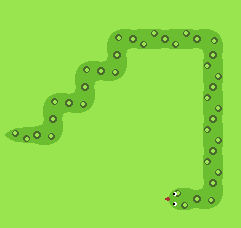
\includegraphics[width=0.4\textwidth]{imgs/lidun.png}
    \caption{\label{Liðun}Hér sést snákurinn liðast.}
\end{wrapfigure}%

Stærsta áskorunin var að láta snákinn líta rétt út þegar hann liðaðist. 
Fyrst þurfti að láta snákinn liðast þar sem hann gerði það ekki í upprunalega verkefninu.
Þetta tók smá hugmyndavinnu og nokkrar tilraunir til að ná réttu, 
en þegar ég var kominn með kassa sem liðuðust fór ég beint í að teikna sprite.
Allt í allt eru sprite-in bara 4, haus, búkur, búkur að beygja og hali.
Stöðurnar sem þessi sprite geta tekið eru samt mjög mörg.
Ég bjó til stóra töflu af öllum stöðum sem hann gæti tekið og tilheyrandi stöðu bæði búts á undann og eftir.
Kóðinn sem útfærði þessar útlitsbreytingar er ekki mjög flottur þar sem hann samanstendur mestmegnis af mörgum if else setningum. 
Hann er samt þess virði því snákurinn liðast núna mjög vel.\\

\begin{wrapfigure}{L}{0.3\textwidth}
    \vspace{-\baselineskip}
    \centering
    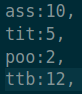
\includegraphics[width=0.3\textwidth]{imgs/stig.png}
    \caption{\label{fig:stig}Gögnin uppsett.}
\end{wrapfigure}%
Næst stærsta verkefnið var að útbúa stigatöfluna. 
Það var hægt að skipta því verkefni niður í þrennt, lestur gagna, skrifun gagna og útlit.
Hér fór ég gegn mínum innri hvötum og byrjaði ekki á að vinna útlitið. 
Fyrst var að finna út hvernig á að lesa úr og skrifa í skrár utan verkefnisins.
Ég byrjaði á að nota JSON skrá til að geyma upplýsingar. 
Vegna þess hve mikið af pökkum og overhead var í kring um JSON hætti ég við að nota það.
Þar sem ég var í raun bara að halda utan um tvær breytur fyrir hverja færslu, 
nafn og stigafjölda, 
ákvað ég frekar að nota einfalt .txt á csv formati.\\


\begin{wrapfigure}{R}{0.4\textwidth}
    \vspace{-\baselineskip}
    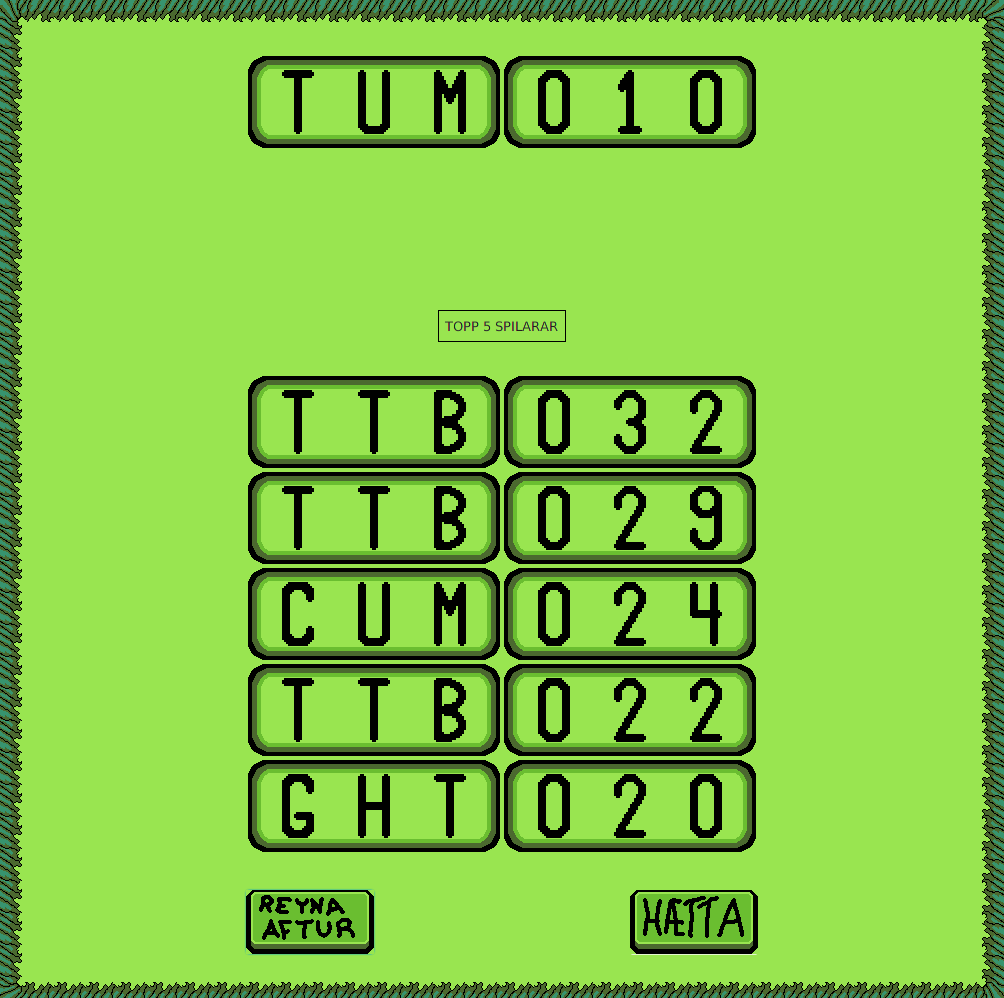
\includegraphics[width=0.4\textwidth]{imgs/stigatafla.png}
    \caption{\label{Mynd:stigatafla}Stigataflan.}
\end{wrapfigure}%
Útlitshlutinn af stigatöflunni var skemmtilegri í útfærslu.
Ég útbjó sérstaka takka og leturgerð til þess að reyna ná gamalds spilakassa stílnum. 
Hvort það heppnaðist er upp til annara komið en mín en það lítur allavega vel út.
Notandi getur þá vistað þriggja stafa nafn eða einkennisstafi, 
og fólk var ekki lengi að búa til "fyndin" nöfn eins og sást á gögnunum á mynd 2. 
Það tók heillangan tíma að finna leið til að vinna úr gögnum eftir að skránum hafði verið þjappað saman í jar skrá.
Að lokum eftir mikið af blóði, svita, tárum og stackoverflow þráðum frá 2013 tókst mér að vinna úr upplýsingum innan úr jar skrá.
Það setti punkt á stigatöfluna og hún gat haldið utan um gögn spilara á milli leikja á meðan hún leit vel út.\\

\begin{wrapfigure}{L}{0.5\textwidth}
    \vspace{-\baselineskip}
    \centering
    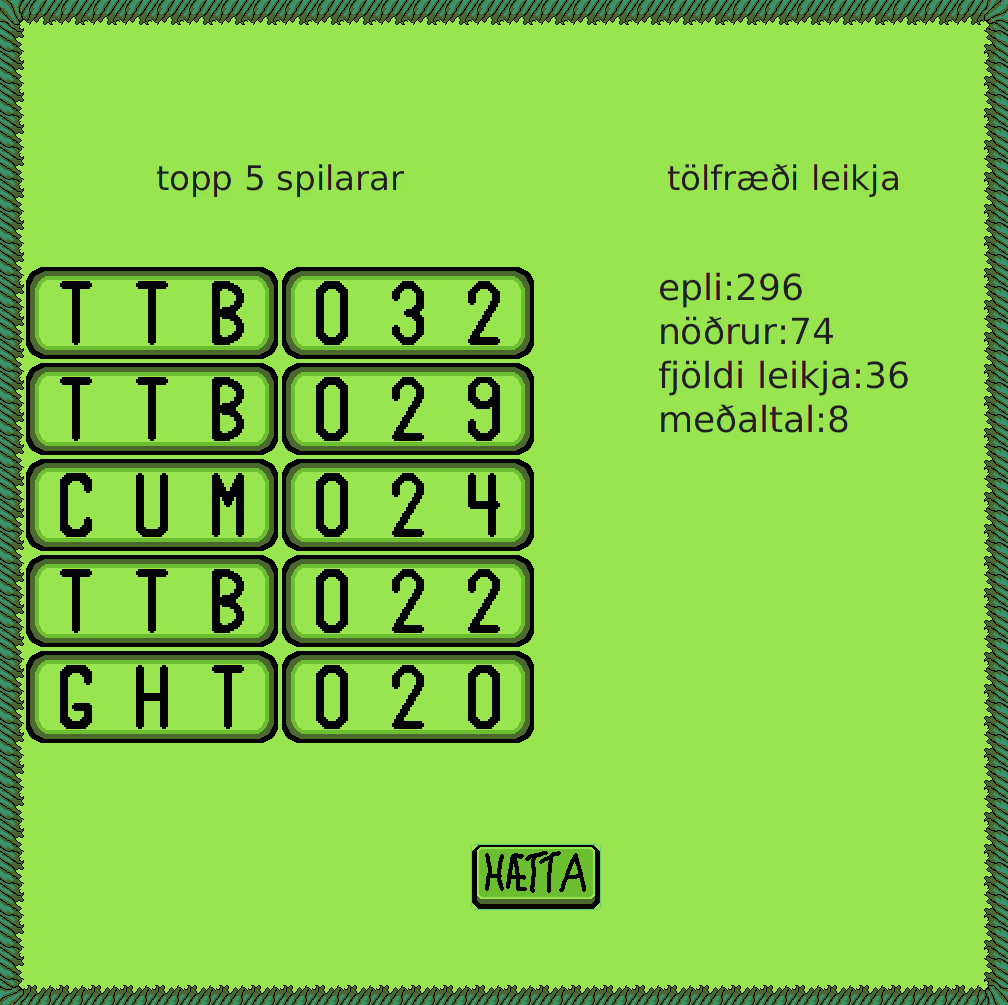
\includegraphics[width=0.5\textwidth]{imgs/stats.png}
    \caption{\label{fig:stats}Tölfræði skjárinn.}
\end{wrapfigure}%
Tölfræði skjárinn eins og ég kalla hann var líka viðbót sem frekar mikil vinna fór í.
Útfærslan á þeim skjá nýtti smá af útlitinu sem fór á stigatöfluskjáinn þannig ég gat nýtt smá af stigatöflukóðanum aftur þar.
Helsta áskorunin hér var að halda utan um upplýsingar innan hvers og eins leiks, 
auk þess sem að halda utan um upplýsingar á milli leikja.
Ég bjó til nýjann vinnsluklasa sem hélt utan um fjölda leikja spilaðra, fjölda óvina, fjölda stiga, fjölda ofurepla (ekki notað) og meðaltal stiga í leikjum.
Það hjálpaði líka voða mikið að vera búinn að útfæra klasa með yfirlit yfir allskonar upplýsingar þegar ég gerði pásu skjáinn.
Hann notaði nýja klasann nema sleppti meðaltali og fjölda leikja.
Svo eftir hvern leik voru upplýsingarnar teknar úr klasanum sem var gerður innan leiks og skrifaðar í skjal ekki ólíkt og með stigafjöldann.

\end{document}